\begin{theo}[Wederzijdse inductie]{Wederzijdse inductie}
    \begin{minipage}{.78\textwidth}
        Als twee spoelen nabij elkaar plaatst worden, zoals in de figuur, dan zal een veranderende stroom in de ene, 
        een emf induceren in de andere. Dus: geïnduceerde emf in een spoel is enevredig met de snelheid van de stroomverandering
        in de andere. Dit noemt men \textbf{wederzijdse inductie} $M$, we noteren
        \begin{equation*}
            M_{21} = \dfrac{N_{2}\Phi_{21}}{I_{1}} 
        \end{equation*}
        met $M_{21}$ de wederzijdse inductiecoefficient en $\Phi_{21}$ de magnetische flux doorheen spoel 2 tegenover de stroom in spoel 1.
        We kunnen dit mengen met de wet van Faraday
    \end{minipage}
    \begin{minipage}{.18\textwidth}
        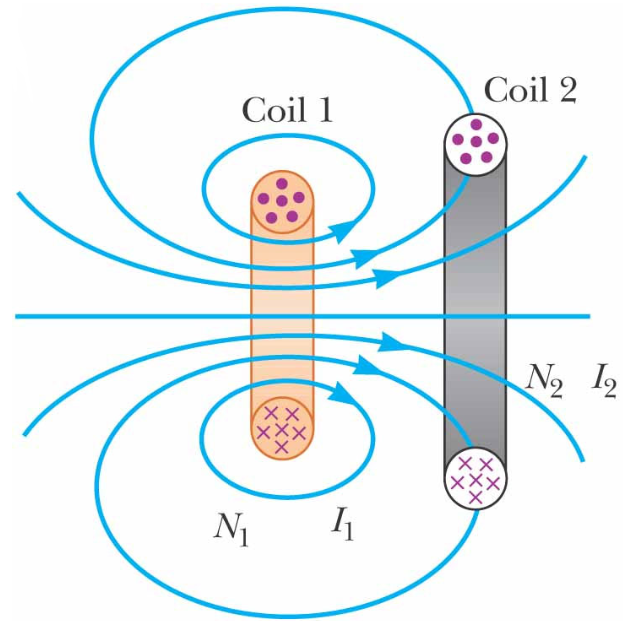
\includegraphics[scale=0.3]{Images/Magnetisme/WederzijdseInductie}
    \end{minipage}
    \begin{equation*}
        \mathcal{E}_{2} = - N_{2}\dfrac{d\Phi_{21}}{dt} = - M_{21}\dfrac{dI_{1}}{dt}
    \end{equation*}
    waarbij nu de verandering in stroom in spoel 1 hebben verbonden aan de emf dat het induceert in spoel 2.  In de algemene situatie is 
    $M = M_{12} = M_{21}$.
\end{theo}

\begin{app}[Wederzijdse inductie van een solenoïde en een spoel]{Wederzijdse inductie van een solenoïde en een spoel}
    De solenoïde is opeengepakt, dus kunnen we veronderstellen dat alle magnetische flux in de solenoïde blijft in de tweede spoel.
    We weten dam wat de flux door deze spoel is, namelijk
    \begin{equation*}
        \Phi_{21} = BA = \mu_{0}\dfrac{N_{1}}{\ell}I_{1}A
    \end{equation*}
    en de wederzijdse inductiecoëfficient
    \begin{equation*}
        M = \dfrac{N_{2}\Phi_{21}}{I_{1}} = \mu_{0}\dfrac{N_{1}N_{2}}{\ell}A
    \end{equation*}
    waarbij we zien dat deze enkel afhangt van de geometrie van het systeem.
\end{app}

\begin{theo}[Zelfinductie]{Zelfinductie}

\end{theo}